\begin{lem}
    \label{lem:manifolds_1}
    For any collection of \(n - m + 1\) vertices \(\{v_\alpha\}_{\alpha=m}^n\)
    in \(\Gamma - \{v_\alpha,  w_\alpha\}_{\alpha=1}^{m-1}\), there exists exactly two edges
    \(e_1 = v_i u_1\) and \(e_2 = v_j u_2\) such that
    \begin{enumerate}[label=(\roman*)]
    \item \(m \leq i, j \leq n\)
    \item \(u_1, u_2 \not \in \{v_\alpha\}_{\alpha=1}^n\cup\{w_\alpha\}_{\alpha=1}^{m-1}\)
    \item Exactly one of the following hold in Figure \ref{fig:lem:manifolds_1}
    \end{enumerate}
    \begin{figure}[h!]
        \centering
        \begin{enumerate*}[label=(\arabic*)]
            \item \label{fig:lem:manifolds_1_1}
            \begin{minipage}{.3\textwidth}
                \centering
                \(v_i = v_j\) \textit{and} \(u_1 \neq u_2\) \\
                \vspace{1em}
                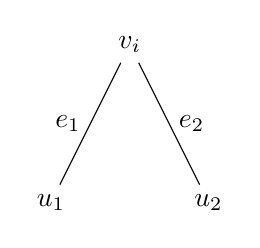
\begin{tikzpicture}
                    \node (vi) at (3, 2) {\(v_i\)};
                    \node (w2) at (2, 0) {\(u_1\)};
                    \node (w3) at (4, 0) {\(u_2\)};

                    \draw (vi) -- (w2) node[midway, left] {\(e_1\)};
                    \draw (vi) -- (w3) node[midway, right] {\(e_2\)};
                \end{tikzpicture} 
            \end{minipage}

            \hspace{3em}

            \item \label{fig:lem:manifolds_1_2}
            \begin{minipage}{.3\textwidth}
                \centering
                \(u_1 = u_2\) \textit{and} \(v_i \neq v_j\) \\
                \vspace{1em}
                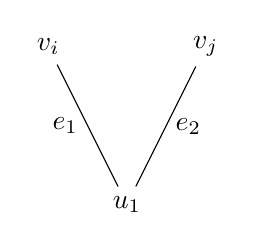
\begin{tikzpicture}
                    \node (vi) at (2, 2) {\(v_i\)};
                    \node (vj) at (4, 2) {\(v_j\)};
                    \node (w2) at (3, 0) {\(u_1\)};

                    \draw (vi) -- (w2) node[midway, left] {\(e_1\)};
                    \draw (vj) -- (w2) node[midway, right] {\(e_2\)};
                \end{tikzpicture}
            \end{minipage}
        \end{enumerate*}
        \caption{Lemma \ref{lem:manifolds_1} possibilities.}
        \label{fig:lem:manifolds_1}
    \end{figure}
\end{lem}

\begin{proof}
    Let \(\{v_\alpha\}_{\alpha=m}^n\) be a collection of \(n - m + 1\) vertices in \(\Gamma - \{v_\alpha, w_\alpha\}_{\alpha=1}^{m-1}\)
    and put a particle at each vertex in \(\{v_\alpha\}_{\alpha=1}^n\).
    The movements of the particles from \((v_\alpha)_{\alpha=1}^{m-1}\) to \((w_\alpha)_{\alpha=1}^{m-1}\)
    correspond to an \((m-1)\)-cube in \(\DConf_n(\Gamma)\).
    Since the configuration space is an \(m\)-manifold without boundary, 
    this \((m-1)\)-cube must border exactly two distinct \(m\)-cubes.
    For this \((m-1)\)-cube to border two \(m\)-cubes,
    there needs to exist two additional mutually exclusive particle movements.
    Let \(v_i, v_j \in \{v_\alpha\}_{\alpha=m}^n\) be the vertices that these particles occupy.
    Since the particle(s) at \(v_i\) and \(v_j\) need to move simultaneously as the particles move from \((v_\alpha)_{\alpha=1}^{m-1}\) to \((w_\alpha)_{\alpha=1}^{m-1}\),
    there exist destination(s) \(u_1\) and \(u_2\) outside the set \(\{v_{\alpha}\}_{\alpha=1}^n \cup \{w_\alpha\}_{\alpha=1}^{m-1}\).
    In order for these additional movements to be mutually exclusive, either \(v_i \neq v_j\) or \(u_1 \neq u_2\) but not both.
\end{proof}